\documentclass[10pt,a4paper]{article}
\usepackage[T1]{fontenc}
\usepackage[scaled]{helvet}
\usepackage{cite}
\usepackage{url}
\usepackage{graphicx}
\usepackage{listings}
\usepackage{float}
\usepackage{amsmath}
\usepackage{listings}
\usepackage{color}
 
\definecolor{dkgreen}{rgb}{0,0.6,0}
\definecolor{gray}{rgb}{0.5,0.5,0.5}
\definecolor{mauve}{rgb}{0.58,0,0.82}
\lstset{ %
  language=Octave,                % the language of the code
  basicstyle=\footnotesize,           % the size of the fonts that are used for the code
  numbers=left,                   % where to put the line-numbers
  numberstyle=\tiny\color{gray},  % the style that is used for the line-numbers
  stepnumber=1,                   % the step between two line-numbers. If it's 1, each line 
                                  % will be numbered
  numbersep=5pt,                  % how far the line-numbers are from the code
  backgroundcolor=\color{white},      % choose the background color. You must add \usepackage{color}
  showspaces=false,               % show spaces adding particular underscores
  showstringspaces=true,         % underline spaces within strings
  showtabs=false,                 % show tabs within strings adding particular underscores
  frame=none,                   % adds a frame around the code
  rulecolor=\color{black},        % if not set, the frame-color may be changed on line-breaks within not-black text (e.g. commens (green here))
  tabsize=4,                      % sets default tabsize to 2 spaces
  breaklines=true,                % sets automatic line breaking
  breakatwhitespace=false,        % sets if automatic breaks should only happen at whitespace
  keywordstyle=\color{blue},          % keyword style
  commentstyle=\color{dkgreen},       % comment style
  stringstyle=\color{mauve},         % string literal style
  escapeinside={\%*}{*)},            % if you want to add LaTeX within your code
  morekeywords={*,...}               % if you want to add more keywords to the set
}
\usepackage{amssymb}
\usepackage{fancyhdr}
\usepackage{lastpage}
\floatstyle{boxed} 
\restylefloat{figure}
\renewcommand*\familydefault{\sfdefault}
\title{Quasi-Linear and Linear Running Time Sorting Algorithms}
\author{David Lynch - david.lynch@raglansoftware.com }
\begin{document}
\maketitle
\begin{abstract}
This article focuses on quasi-linear or $O(n log n)$ running time algorithms in a lot of detail. This article will be really important to know well when it comes to your second assignment. We will spend a little less time looking at linear or $O(n)$ running time algorithms.
\end{abstract}
\section{Quasi-Linear Sorting}
This section discusses two common sorting algorithms that sort in {\bf nearly} linear time. That is, a time complexity that is not quite as good as linear time, but not quite as bad as polynomial time. 
\subsection{Heap Sort}
Heap-sort is an $O(n log n)$ running time algorithm that sorts {\bf in place} This is the first sorting algorithm whereby a complex tree-based data structure, or {\bf heap} is used to facilitate our algorithm. We will explore heap-sort itself, but also heaps and how they are useful for implementing priority queues. Note that {\bf it} heap is a hugely overloaded term. Do not confuse this particular flavour of heap with that associated with memory allocation.   
\subsubsection{Heap}
A {\bf binary heap} is an array object that we can view as a nearly complete binary tree. The tree is full on all levels except for the lowest level which is filled from the left up to some point. Figure \ref{heap} shows the tree diagrammatically and figure \ref{heaparray} shows how we can represent this using a one-dimensional array. 
\begin{figure}
\caption{Tree Representation of a Heap \cite{INTROALG}}
\begin{center}
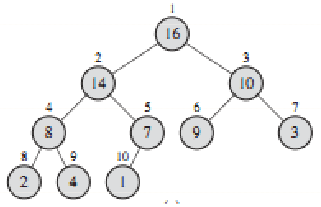
\includegraphics[scale=0.43]{../images/heap.png}
\label{heap}
\end{center}
\end{figure}
\begin{figure}
\caption{Array Representation of a Heap \cite{INTROALG}}
\begin{center}
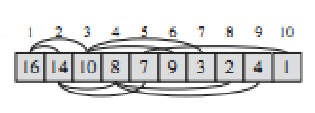
\includegraphics[scale=0.43]{../images/heaparray.png}
\label{heaparray}
\end{center}
\end{figure}
\subsubsection{The Heap Property}
There are two kinds of heap property. In a {\bf max-heap} for every node $i$ other than the root $A[Parent(i)]>= A[i]$. In other words the value of a node is at most the value of its parent. The largest element in a maximum heap is its root and the sub tree will contain no value larger than the root itself. A {\bf min-heap} is organized in exactly the opposite way. For $i$ other than the root $A[Parent(i)]<= A[i]$ i.e. the value of a node is at least equal to its parent. Heap sort uses max-heaps, but keep min-heaps in mind as they are very useful for {\bf priority queues}, something which we will look at later. As with any tree structure the height of the tree $h$ is the number of edges on the longest simple downward path from the root to a null terminator. 
\subsubsection{Heap Operations}
Basic heap operations run in a time that is at most proportional to the height of the tree and therefore are $O(n log n)$ operations. Figure \ref{heapops} illustrates the operations that we must implement on our heap. 
\begin{figure}
\caption{Operations on a Heap}
\begin{center}
\begin{tabular}{| l | l | l | }
\hline 
Name & Description & Running Time  \\
\hline
MAX-HEAPIFY & Apply the heap property & $O(n log n)$ \\
BUILD-MAX-HEAP & Build a full heap & $O(n)$ \\
HEAPSORT & Sort the array in place & $O(n log n)$ \\
HEAP-INSERT & Insert into a heap & $O(n log n)$ \\
HEAP-EXTRACT-MAX & Remove the max value from a heap & $O(1)$ \\
HEAP-INCREASE-KEY & Bump priority & $O(n log n)$  \\
HEAP-MAXIMUM & Top of heap & O(1) \\
\hline
\end{tabular}
\label{heapops}
\end{center}
\end{figure}
\begin{figure}
\caption{Maintaining the heap property}
\begin{center}

\begin{lstlisting}
PARENT(i)
	return FLOOR(i/2)
\end{lstlisting}
	
\begin{lstlisting}
LEFT(i)
	return 2*i
\end{lstlisting}

\begin{lstlisting}
RIGHT(i)
	return 2*i + 1
\end{lstlisting}

\begin{lstlisting}
MAX-HEAPIFY(A, i)
l = left(i)								# left child	
r = right(i)							# right child
if l <= A.heapSize and A[l]>A[i] 	
     largest = 1						# Largest at root
else 
	 largest = i						# Largest is new element
if r <= A.heapSize & A[r]>A[largest]
	largest = r							# Greater than largest thus far
if largest != i					
	exchange A[i] with A[largest]			
	MAX-HEAPIFY(A, largest)				# Recurse down the tree
\end{lstlisting}


\begin{lstlisting}
BUILD-MAX-HEAP(A)
A.heapsize = A.length 
for i = [A.length/2] downto 1
	MAX-HEAPIFY(A, i) 
\end{lstlisting}

\label{heapify}
\end{center}
\end{figure}
Firstly we  must build our maximum heap from an list of unsorted input keys. Figure \ref{heapify} shows the listing for this. The loop invariant for BUILD-MAX-HEAP states that each node $i+1, i+2,...,n$ is the root of a maximum heap. As an exercise, work through how the loop invariant holds true at initialization, maintenance and termination for yourself. Don't move on until you understand this. The time required by MAX-HEAPIFY when called on a node of height $h$ is $O(h)$.
\subsubsection{Sorting}
The heap-sort algorithm is actually quite simple when compared to the maintenance of the data-structure it uses. Figure \ref{heapsort} shows the listing for the heap-sort algorithm. The essence of the algorithm is to start with building a maximum heap on the array. We continually swap the $ith$ element in the array with the first element in the array. Thereafter, we ensure that the heap property is maintained, as it may have been violated by the exchange. 
\begin{figure}
\caption{Sorting}
\begin{center}
\begin{lstlisting}
HEAPSORT(A)
	BUILD-MAX-HEAP(A)
	exchange A[1] with A[i]
	A.heap-size = A.heap-size-1
	MAX-HEAPIFY(A, 1) 
\end{lstlisting}
\label{heapsort}
\end{center}
\end{figure}

\begin{figure}
\caption{(a) is the max-heap structure just after BUIL-MAX-HEAP. The remainder {\it b-j} are snaps of the max-heap just after each all of MAX-HEAPIFY\cite{INTROALG}}
\begin{center}
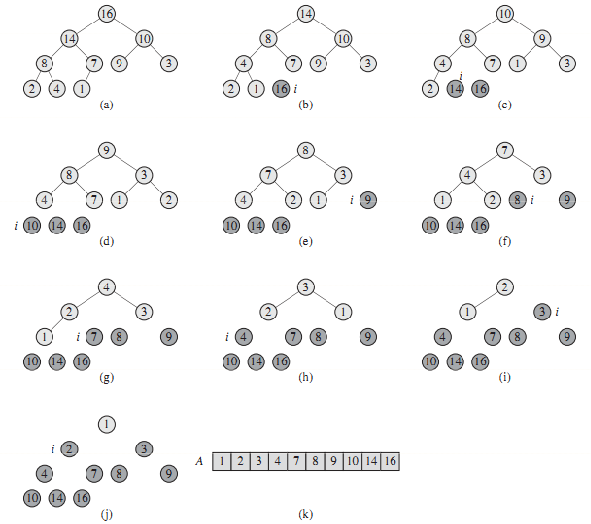
\includegraphics[scale=0.58]{../images/heapsort.png}
\label{heap}
\end{center}
\end{figure}


\subsubsection{Priority Queues}
In practice a good implementation of quick-sort will win out over heap sort. The heap data structure itself is commonly uses as an efficient priority queue. Priority queues are useful, for example, in situations where we need to maintain a queue of jobs from which some candidate job is selected as the next job based on a set of criteria. 
\newline\newline
A priority queue is a data structure for maintaining a set $S$ of elements, each with an associated key value. In a priority situation, we are concerned about addition (figure \ref{heapinsert}) and extraction (figure \ref{heapremove}) elements while maintaining some order. Furthermore, it is very desirable for us to optimize the running time of both the insertion and deletion mechanism. Insertion into the set $S$ of an element with a specific key must focus on insertion of the the key into its correct slot of priority. To do this we essentially increase the size of the underlying heap array, and recursively {\it increase the key} by means of a series of parent-swaps. We break when the new key has been inserted into the correct position. For removal, we simply take the first element of the array, decrease the heap size and maintain the heap property on the remaining array. 



\begin{figure}
\caption{Extracting maximum key from the heap \cite{INTROALG}}
\begin{center}

\begin{lstlisting}
HEAP-MAXIMUM(A)
	return A[1]
\end{lstlisting}

\begin{lstlisting}
HEAP-EXTRACT-MAX(A)
if A.heapSize < 1 
	error heap underflow
max = A[1]
A[1] = A[A.heapSize]
A.heapSize = A.heapSize -1 
MAX-HEAPIFY(A, 1)
return max
\end{lstlisting}
\label{heapremove}
\end{center}
\end{figure}




\begin{figure}
\caption{Inserting into the heap \cite{INTROALG}}
\begin{center}
\begin{lstlisting}
HEAP-INCREASE-KEY(A,i,key)
  if key < A[i]
        error new key is smaller than current
 A[i] = key
 while i > 1 and A[Parent(i)] < A[i]
        exchange A[i] with A[Parent(i)]
 i = Parent(i)
\end{lstlisting}

\begin{lstlisting}
MAX-HEAP-INSERT(A, key)
A.heapSize = A.heapSize + 1
A[A.heapSize] = NIL
HEAP-INCREASE-KEY(A, A.heapSize, key)
\end{lstlisting}
\label{heapinsert}
\end{center}
\end{figure}


\subsection{Quicksort}
The worst case running time for quicksort is $O(n^2)$ but is still often the best practical choice for sorting due to its remarkably efficient average running time of $O(nlogn)$. The algorithm breaks down as follows
\subsubsection{Divide}
Partition the array $A[p..r]$ into two possibly empty sub-arrays $A[p..q-q]$ and $A[q+1..r]$ such that each element of $A[p..q-1]$ is less than or equal to each of $A[q+1..r]$.
\subsubsection{Conquer}
Sort the two sub arrays $A[p..q-1]$ and $A[q+1..r]$ recursively. 
\subsubsection{Combine}
Sub arrays are already sorted, so in contrast to merge-sort, there is nothing to do here. 

\begin{figure}
\caption{Sorting}
\begin{center}

\begin{lstlisting}
PARTITION(A,p,r)
x = A[r] // pivot
i = p -1 
for j = p to r -1 
	if A[j]<=x then
		i = i +1
		exchange A[i] with A[j]
	exchange A[i+1] with A[r]		
return i+1		
\end{lstlisting}



\begin{lstlisting}
RANDOMIZED-PARTITION(A, p, r)
i = random(p,r)
exchange A[r] with A[i]
return PARTITION(A,p,r)
\end{lstlisting}


\begin{lstlisting}
RANDOMIZED-QUICKSORT(A,p,r)
if p < r 
	q = RANDOMIZED-PARTITION(A,p,r)
	RANDOMIZED-QUICKSORT(a, p, q - 1)
	RANDOMIZED-QUICKSORT(a, q+1, r)
\end{lstlisting}
\label{rndquicksort}
\end{center}
\end{figure}

\subsubsection{Loop Invariant}
At each iteration of the loop of lines 4-7 of the partition function for any array index k the loop invariant is as follows. If $p<=k <= i$, then $A[k] <= x$. Otherwise, if $i+1 <= k <= (j-1)$, then $A[k]>x$. Lastly, if $k = r$, then $A[k] = x$. Work through this yourself outlining how this holds at initialization, maintenance and termination.  

\subsubsection{Running Time}
Running time is dependent on whether the partitioning is {\bf balanced} or {\bf unbalanced} which depends in turn on which elements are being used for partitioning. If balanced, the algorithm can run as fast as merge-sort, but if unbalanced it can run as slow as insertion sort. Worst case partitioning is the case where the partition routine produces one array of $n-1$ elements and another array of zero elements. This evaluates to $O(n^2)$ and happens if the input array is already sorted. Best case partitioning produces the most even possible split of elements, and produces problems of no more than $n/2$ in size. Average case is much closer to best case than it is to worst case. When quicksort is run on a random input array the partitioning is unlikely to happen in the same way at every level. In other words, we will have some balanced, and some unbalanced splits. We cannot generally assume that all permutations of input numbers are equally likely. 
\newline\newline
As with randomized merge-sort, we can inject randomness into the selection of the pivot. See figure \ref{rndquicksort} for an illustration. 

\section{Linear Time Sorts}
So far we have seen sorts that comprise of comparisons between the input elements. $\Omega(n log n)$, or linearithmic time is the lower bound of performance for all comparison sorts. However, there are some algorithms that run in linear time. Two of these are discussed here. 
\subsection{Counting Sort}
Counting sort is a stable sort that assumes that each of the $n$ input elements is an integer in the range $0$ to $k$ for some integer $k$. This sort runs in $\Theta(n)$ time. This algorithm is quite simple in its execution. For each input $x$ in an array $A$ the number of elements less than $x$ is determined. Thereafter, $x$ is place directly into its position in the output array. See figure \ref{counting} for a listing.   
\begin{figure}
\caption{Counting Sort \cite{INTROALG}}
\begin{center}
\begin{lstlisting}
let C[0..k] be a new array
for i = 0 to k 
	c[i]=0
for j = 1 to A.length 
	C[A[j]]=C[A[j]]+1
# C[i] has i number of elements
for i = 1 to k
	C[i] = C[i]+C[i-1]
# C[i] has less than or equal to i elements
for j = A.length downto 1
	B[C[A[j]]] = A[j]
	C[A[j]]=C[A[j]]-1
\end{lstlisting}
\label{counting}
\end{center}
\end{figure}


\subsection{Radix Sort}
This is also a non-comparative integer sort algorithm. Keys are grouped by the individual keys that share the same {\bf significant position} and value. Two classes of radix sort exist, {\bf least significant digit} and {\bf most significant digit}. Radix sort has $O(kn)$ running time where $k$ is the average length of the key. 
\newline\newline
The algorithm works by taking the most (or least) significant digit of each key. Next, we group those based on digit but otherwise keep the original ordering of the keys. At each iteration, we do a stable sort of the group of keys we are focused on. We repeat this with the following more or least significant digits until we run out of digits. Figure \ref{radix} illustrates this with a least-to-most significant digit sort. 
\begin{figure}
\caption{Radix Sort Example \cite{INTROALG}}
\begin{center}
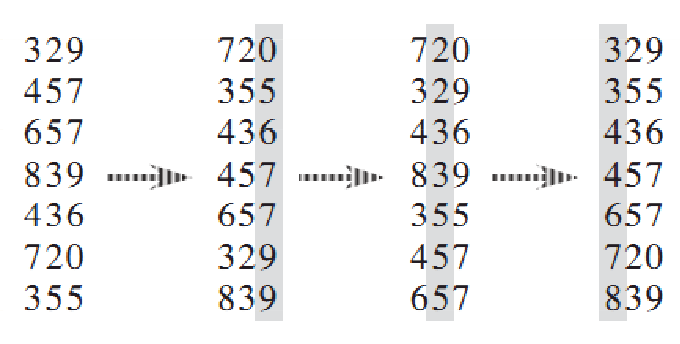
\includegraphics[scale=0.43]{../images/radix-sort.png}
\label{radix}
\end{center}
\end{figure}
\newline\newline
This article marks the end of our formal discussion of data-structures and algorithms. For those interested in more complex structures and their use cases, or more detail, I suggest following up in \cite{INTROALG}. In studying these sections, I reiterate the recommendation to fully implement your own flavours of all the data-structures and algorithms discussed. Going into the exam having done this will leave you in a very strong position. Some of the information in here is quite terse when compared to the other notes, so review these articles slowly until you understand each caveat of each algorithm. A significant portion of the exam focuses on this and the previous two articles. 
\bibliography{../biblio/techfundamentals.bib}{}
\bibliographystyle{plain}
\begin{center}
\end{center}
\end{document}
